Nessa sessão apresento os principais resultados referentes aos métodos que
apliquei aos dados de previsão. 

\subsection{Analisando a Média}

Para esse método, o teste de Ljung-Box indicou que existe correlação temporal,
i.e, autocorrelação. O valor do p-valor ficou extremamente próximo de $0$, o
que indica que a hipótese nula é rejeitada a um nível $5\%$. Além disso, o
valor do nosso erro MASE ficou maior que $1$, sendo equivalente a $1.16$, o
que significa que ele não melhora a estimativa da média de todos os dados e
estimar baseado nessa média.

De fato, esse não é um bom preditor para esses dados, visto que eles carregam
muita variação. Entretanto, ele estabelece um limite mínimo de qualidade para
os próximos métodos para esse conjunto de dados. Confira a Figura
\ref{mean-estimation}.

\subsection{Analisando a Regressão Linear}

O método de Regressão Linear também não foi capaz de capturar a variabilidade
dos nossos dados. Nesse caso, fiz duas predições, uma que incluísse as
variáveis indicadoras dos meses, e outra que não, apenas as variáveis já
citadas anteriormente. Nos dois casos, os resultados não foram tão bons. 
Nos dois casos, o teste de Ljung-Box evidenciou que os resíduos possuiam
autocorrelação, o que significa que o modelo não foi capaz de capturar toda a
informação temporal contida nos dados. Acredito que isso se deva ao fato da
grande variabilidade já citada. Alguma transformação necessitaria ter sido
feita nesses dados a fim de resolver esse problema. Entretanto, deixo esse
fato para futuros trabalhos.

Sobre os resultados, quando considerei os meses como variáveis do meu
problema, o erro calculado foi de $1.01$. Esse resultado já foi melhor do que
a média, mas ainda não capturou dados suficientes sobre os dados. Já o
coeficiente de determinação foi de $0.5$, relativamente baixo, o que evidencia
que essas variáveis não foram boas para estimar minha série temporal. Acredito
que isso se deva à falta de algum parâmetro e os valores faltantes em cada
variável, que somados podem ter influenciado negativamente os dados. 

Quando retirei as variáveis sobre os meses, obtive um resultado do erro de
$0.96$, meu primeiro valor menor do que um nesse sentido. Entretando, o
coeficiente de determinação foi de $0.42$, bem inferior ao anterior. Isso é
explicado pelo seguinte fato. Adicionar variáveis não reduz o coeficiente de
determinação, pois se reduzisse, bastaria colocar o parâmetro correspondente
como $0$. Nesse sentido, não acredito que o resultado anterior foi melhor.
Confira o resultado desse teste, sem as variáveis indicadoras, na Figura
\ref{linear-estimation}. 

\subsection{Analisando a Suavização Exponencial}

Esse método também não foi feliz para modelar o problema. Nesse caso, o
problema é possivelmente na quantidade de informações, que dificulta a
estimação. O método teve o pior desempenho no cálculo do erro, apesar de ter
reduzido os valores das estatísticas de Ljung-Box, apesar de que ainda o teste
considerou os resíduos autocorrelacionados. Na imagem \ref{exp-estimation},
coloquei todos os valores estimados pelo modelo, e os valores estimados para o
conjunto de teste. Os resíduos apresentaram o melhor resultado de encaixe dos
dados. Uma possível maneira de corrigir esse problema seria considerar os
valores de concentração por mês. 

O valor do erro foi de $1.28$.

\begin{figure*}
    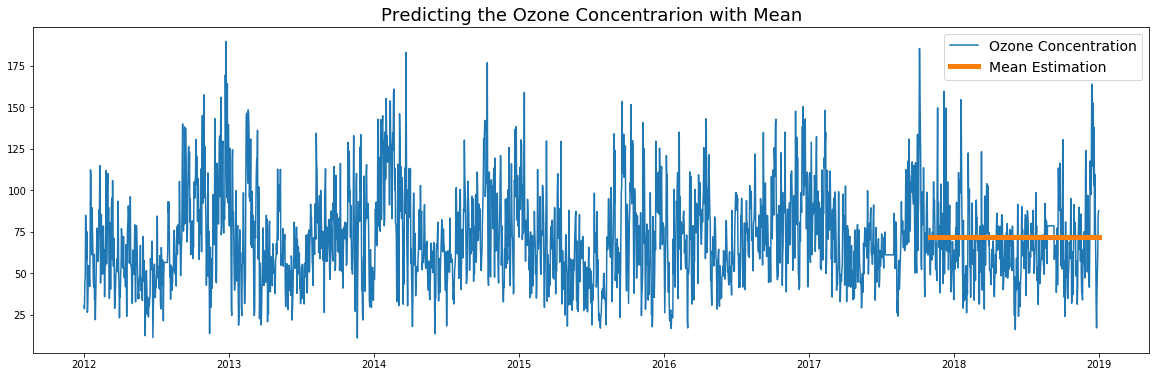
\includegraphics[width=\linewidth]{img/graphic5.png}
    \caption{Previsão utilizando o método da Média}
    \label{mean-estimation}
\end{figure*}

\begin{figure*}
    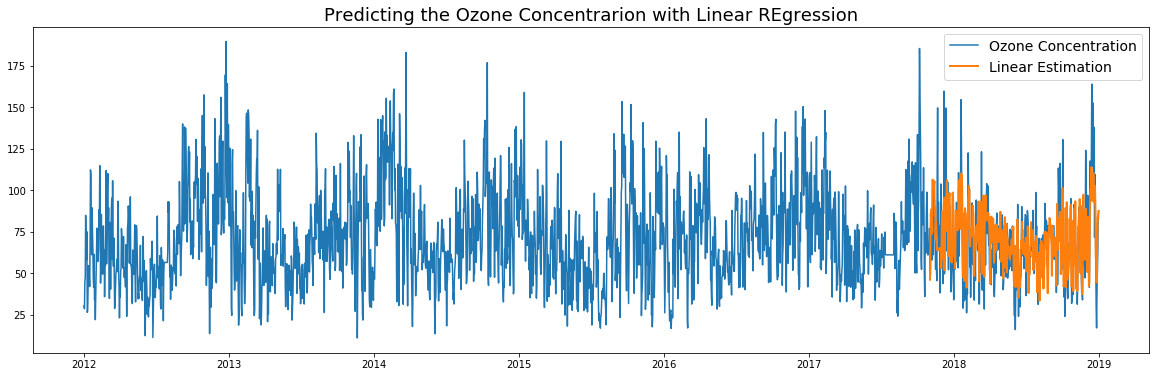
\includegraphics[width=\linewidth]{img/graphic6.png}
    \caption{Previsão utilizando o método de Regressão Linear}
    \label{linear-estimation}
\end{figure*}

\begin{figure*}
    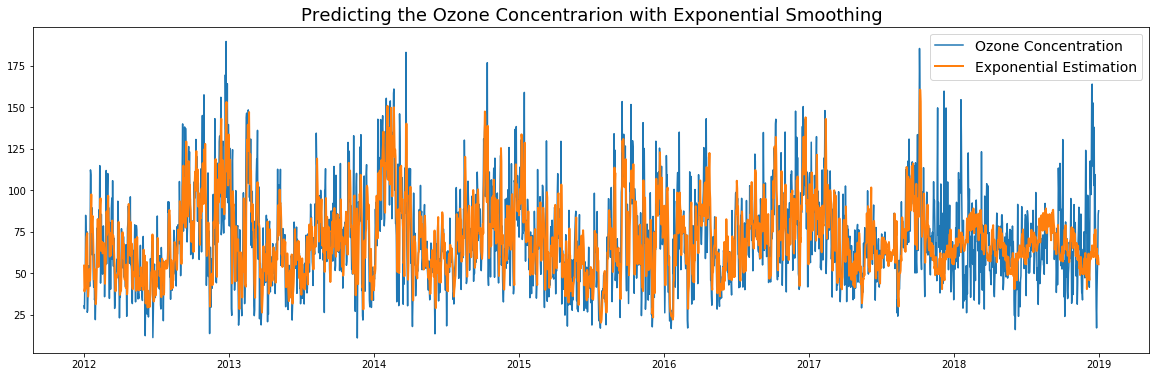
\includegraphics[width=\linewidth]{img/graphic7.png}
    \caption{Previsão utilizando o método da Suavização Exponencial}
    \label{exp-estimation}
\end{figure*}

\subsection{Discussões sobre os Resultados}

Os resultados não foram bons como esperado antes do problema ser enunciado,
entretanto, acredito que o processo tenha sido sólido o suficiente para a
extensão para melhorar as simulações numéricas e a teoria sobre outros métodos
seja enunciada de maneira natural. 

Os métodos apresentados por séries temporais, aqui neste trabalho, se
mostraram não suficientes para explicar o comportamento da concentração de
ozônio, apenas com esse banco de dados. Acredito que outros métodos devam ser
aplicados em ordem de obter resultados melhores. 

Entretanto, um resultado ficou claro. Podemos observar, principalmente no
método de Regressão Linear, que muitos dos dias apresentam quantidade de
ozônio maior do que $80$. Esse valor chave é definido pelo Boletim de
Qualidade do Ar, como máximo de ozônio para que o ar seja considerado bom.
Entretanto, nenhum valor superou o valor de $160$, atingindo a qualidade de ar
inadequada. Dessa forma, as políticas esperadas de atuação não precisam ser
intensas, apenas controles bem localizados. 

\subsection{Futuros Trabalhos}

\begin{enumerate}
    \item Melhorar a forma de inserir dados novos no lugar de dados faltantes.
    Para isso, propor métodos de regressão linear ou inferência causal;
    \item Melhorar a regressão linear, fazendo diferentes testes com variáveis
    fora do banco de dados, como, por exemplo, produção em indústrias locais; 
    \item Aplicar transformações na série temporal de estudo, afim de obter
    melhores resultados;
    \item Aplicar testes da importância dos \textit{outliers} nos modelos e
    retirá-los, quando evidente.
    \item Fazer os mesmos estudos, só que no sentido mais amplo, mensal. 
\end{enumerate}